\documentclass{standalone}
\usepackage{tikz,pgfplots,pgfplotstable}
\usepackage{xcolor}
\pgfplotsset{compat=newest}
\usetikzlibrary{positioning}
\usepgfplotslibrary{fillbetween}
\usetikzlibrary{shapes}

\newcommand{\smilename}{SMiLe$^{*}$}
\newcommand{\vsmile}{VarSMiLe}
\newcommand{\pfone}{pf1}
\newcommand{\pften}{pf10}
\newcommand{\pftwenty}{pf20}
\newcommand{\leaky}{Leaky}
\newcommand{\mpbayes}{Exact Bayes}
\newcommand{\mpone}{MP1}
\newcommand{\mpten}{MP10}
\newcommand{\mptwenty}{MP20}
\newcommand{\nassarten}{Nas10$^{*}$}
\newcommand{\nassartwelve}{Nas12$^{*}$}
\newcommand{\nassartenoriginal}{Nas10 original}
\newcommand{\nassartwelveoriginal}{Nas12 original}
\newcommand{\mporiginalone}{SOR1}
\newcommand{\mporiginalten}{SOR10}
\newcommand{\mporiginaltwenty}{SOR20}
\newcommand{\smileoriginal}{SMiLe}


\definecolor{mp1color}{rgb}{0.15,0.58,1}
\definecolor{mp10color}{rgb}{0,1,1}

\tikzset{
    %font = \scriptsize,
    font = \small,
    %font = \large,
    actualpcstyle/.style = {anchor = east, rotate = 90, isosceles triangle, fill = red!90!black, draw = none, inner sep = 1},
    mustyle/.style = {anchor = east, rotate = 90, isosceles triangle, fill = blue!80!black, draw = none, inner sep = 1, minimum width=0.3cm},
    smile/.style = {orange!90, thick},
    smileextended/.style = {red!60!black, thick},
    pf1/.style = {lime, thick},
    pf20/.style = {green!40!black, thick},
    leaky/.style = {gray, thick},
    bayesfilter/.style = {black, thick},
    gsor1/.style = {mp1color, thick},
    gsor20/.style = {blue, thick},
    tsor1/.style = {mp1color, thick},
    tsor10/.style = {mp10color, thick},
    tsor20/.style = {blue, thick},
    gnassarJN/.style = {magenta, thick},
    gnassarNatN/.style = {violet!90!black, thick},
    gnassarJNOriginal/.style = {magenta, thick, dashed},
    gnassarNatNOriginal/.style = {violet!90!black, thick, dashed},
    gsorOriginal1/.style = {green!95!black, thick},
    gsorOriginal20/.style = {mp10color, thick},
    tsorOriginal1/.style = {green!95!black, thick},
    tsorOriginal20/.style = {mp10color, thick},
    smileOriginal/.style = {orange!90, thick},
    %
    GNassarNatN_Sgmpositive/.style =  {orange!90, thick},
    GNassarNatN_Sgmnegative/.style =  {blue, thick},
    GNassarNatN_Sshpositive/.style =  {orange!90, thick},
    GNassarNatN_Sshnegative/.style =  {blue, thick},
    GParticleFilter_Sgmpositive/.style =  {orange!90, thick},
    GParticleFilter_Sgmnegative/.style =  {blue, thick},
    GParticleFilter_Sshpositive/.style =  {orange!90, thick},
    GParticleFilter_Sshnegative/.style =  {blue, thick},
    %
    GNassarNatN_Sgm/.style =  {green!40!black, thick},
    GNassarNatN_Ssh/.style =  {mp1color, thick},
    GParticleFilter_Sgm/.style =  {green!40!black, thick},
    GParticleFilter_Ssh/.style =  {mp1color, thick},
}
\pgfplotsset{
    legend style = {draw = none},
    colorbar/width = 6pt,
}
\newcommand{\plotwithquantiles}[2]{
    \addplot[draw = none, name path=lower] table[x = x, y expr = \thisrow{#1_mean} - \thisrow{#1_se}] {#2};
    \addplot[draw = none, name path=upper] table[x = x, y expr = \thisrow{#1_mean} + \thisrow{#1_se}] {#2};
    \addplot[#1, opacity = .4] fill between [of=lower and upper];
    \addplot[#1] table[x = x, y = #1_mean] {#2};
}
\newcommand{\trimleft}[1]{
    \begin{tikzpicture}[trim axis left]
        #1
    \end{tikzpicture}
}
\newcommand{\trimright}[1]{
    \begin{tikzpicture}[trim axis right]
        #1
    \end{tikzpicture}
}
\newcommand{\trimboth}[1]{
    \begin{tikzpicture}[trim axis right, trim axis left]
        #1
    \end{tikzpicture}
}
\newcommand{\heatmap}[2]{
    \begin{axis}[
        view = {0}{90},
        xtick = {-4,-3,-2.3,-2,-1.3,-1},
        xmin = -4.2, xmax = -.85,
        ymin = \ymin.2, ymax = .9,
        yticklabel = \empty,
        xticklabels = {$10^{-4}$,,,$10^{-2}$,},
        tick style = {white},
        xlabel = $p_c$,
        point meta min = -4., point meta max = \zmax,
        colormap/viridis,
        width = 4.8cm, height = 4.8cm,
        #2
        ]
        \addplot[matrix plot*, point meta = explicit, mesh/rows = \rows, mesh/cols = \cols]  table[x expr = log10(\thisrowno{1}),
              y expr = log10(\thisrowno{0}),
              meta expr = log10(\thisrowno{2})] {#1};
              \draw[white] (-4, \ymin.3) -- (-4, \ymin.05);
              \draw[white] (-2, \ymin.3) -- (-2, \ymin.05);
              \draw[white] (-4.3, -1) -- (-4.05, -1);
              \draw[white] (-4.3, 0) -- (-4.05, -0);
              \draw[white] (-4.3, -2) -- (-4.05, -2);
              \draw[white] (-4.3, .699) -- (-4.05, .699);
    \end{axis}
}

\newcommand{\heatmapblack}[2]{
    \begin{axis}[
      axis background/.style={fill=black},
        view = {0}{90},
        xtick = {-4,-3,-2.3,-2,-1.3,-1},
        xmin = -4.2, xmax = -.85,
        ymin = \ymin.2, ymax = .9,
        yticklabel = \empty,
        xticklabels = {$10^{-4}$,,,$10^{-2}$,},
        tick style = {white},
        xlabel = $p_c$,
        point meta min = -4., point meta max = \zmax,
        colormap/viridis,
        width = 4.8cm, height = 4.8cm,
        #2
        ]
        \addplot[matrix plot*, point meta = explicit, mesh/rows = \rows, mesh/cols = \cols]  table[x expr = log10(\thisrowno{1}),
              y expr = log10(\thisrowno{0}),
              meta expr = log10(\thisrowno{2})] {#1};
              \draw[white] (-4, \ymin.3) -- (-4, \ymin.05);
              \draw[white] (-2, \ymin.3) -- (-2, \ymin.05);
              \draw[white] (-4.3, -1) -- (-4.05, -1);
              \draw[white] (-4.3, 0) -- (-4.05, -0);
              \draw[white] (-4.3, -2) -- (-4.05, -2);
              \draw[white] (-4.3, .699) -- (-4.05, .699);
    \end{axis}
}

\usepackage{multirow}
\usetikzlibrary{calc}
\usepackage{adjustbox}

\usepackage{amsmath}
\newcommand\xstartingrec{-1}
\newcommand\ystartingrec{-3}
\newcommand\sizerec{1}

\newcommand\stepgrid{1.25}
\newcommand\startlowleft{0.75}
\newcommand\stoplowright{4.25}
\newcommand\stophighright{5.25}

\usetikzlibrary{snakes}

\begin{document}

\begin{minipage}{11cm}
\begin{tabular}{ll}
  \textbf{A} \\
  \hspace{0.5cm}
    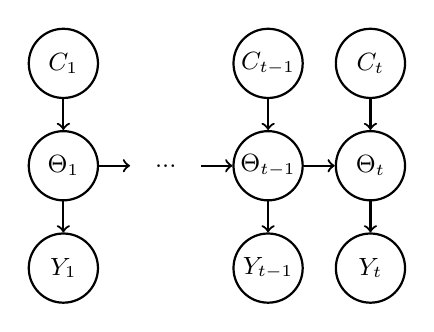
\begin{tikzpicture}
        [
        every node/.style = {circle, minimum width = 2.5em, draw, inner sep = 1},
        node distance = 1.3cm, font = {\small}, thick]
        \node (h) at (0, 0) {$C_t$};
        \node (thetat) [below of=h] {$\Theta_t$};
        \node (thetatminus1) [left of=thetat] {$\Theta_{t-1}$};
        \node (hminus1) [above of=thetatminus1] {$C_{t-1}$};
        \node (x) [below of=thetat] {$Y_t$};
        \node (xminus1) [below of=thetatminus1] {$Y_{t-1}$};
        \node (dots) [draw=none, left of =thetatminus1] {...};
        \node (theta1) [left of=dots] {$\Theta_{1}$};
        \node (h1) [above of=theta1] {$C_{1}$};
        \node (x1) [below of=theta1] {$Y_1$};
        \draw[->] (h) -- (thetat);
        \draw[->] (thetatminus1) -- (thetat);
        \draw[->] (thetat) -- (x);
        \draw[->] (thetatminus1) -- (xminus1);
        \draw[->] (hminus1) -- (thetatminus1);
        \draw[->] (h1) -- (theta1);
        \draw[->] (theta1) -- (x1);
        \draw[->] (theta1) -- (dots);
        \draw[->] (dots) -- (thetatminus1);
    \end{tikzpicture}
    &
    \hspace{0.2cm}
    \parbox[b]{0.3\textwidth}{
    \begin{minipage}{.3\textwidth}
    \begin{equation*}
    \begin{aligned}
    & C_1 = 1 \\
    & C_t \sim \text{Bernoulli}(p_c) \\
    & \Theta_t| \{ C_t = 1 \} \sim \pi^{(0)}(.) \\
    & \Theta_t| \{ C_t = 0 \} = \Theta_{t-1}\\
    & Y_t| \{ \Theta_{t}=\theta \} \sim P_{Y}(. | \theta)\,
    \end{aligned}
  \end{equation*}
    \end{minipage}
    \vspace{10mm}}
    \\
    \textbf{B}\\
     \hspace{1cm}
       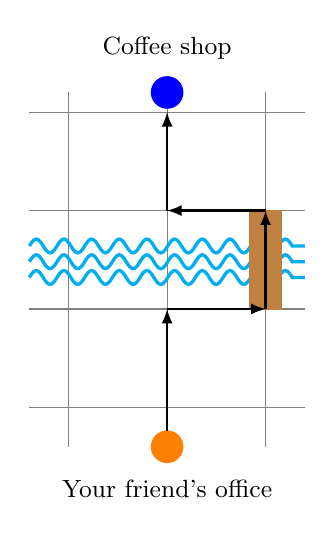
\begin{tikzpicture}
         \draw[step=\stepgrid cm,color=gray] (\startlowleft,\startlowleft) grid (\stoplowright,\stophighright);
         % --- Blue circle
         \draw [blue,fill] (2*\stepgrid , \stophighright) circle [radius=0.2] node [black,above=0.3] {Coffee shop};
         % --- Orange circle
         \draw [orange,fill] (2*\stepgrid , \startlowleft) circle [radius=0.2] node [black,below=0.3] {Your friend's office};
         % --- River
         \draw[cyan, very thick, snake=coil,segment aspect=0] (\startlowleft,2*\stepgrid+0.4)   -- (\stoplowright,2*\stepgrid+0.4);
         \draw[cyan, very thick, snake=coil,segment aspect=0] (\startlowleft,2*\stepgrid+0.6)   -- (\stoplowright,2*\stepgrid+0.6);
         \draw[cyan, very thick, snake=coil,segment aspect=0] (\startlowleft,2*\stepgrid+0.8)   -- (\stoplowright,2*\stepgrid+0.8);
         % --- Detour Bridge
         \draw[brown, fill] (3*\stepgrid - 0.2, 2*\stepgrid) rectangle (3*\stepgrid + 0.2, 3*\stepgrid);
         % --- Path
         \draw[->, >=latex, thick] (2*\stepgrid, \startlowleft+0.2)  -- (2*\stepgrid, 2*\stepgrid);
         \draw[->, >=latex, thick] (2*\stepgrid, 2*\stepgrid)  -- (3*\stepgrid, 2*\stepgrid);
         \draw[->, >=latex, thick] (3*\stepgrid, 2*\stepgrid)  -- (3*\stepgrid, 3*\stepgrid);
         \draw[->, >=latex, thick] (3*\stepgrid, 3*\stepgrid)  -- (2*\stepgrid, 3*\stepgrid);
         \draw[->, >=latex, thick] (2*\stepgrid, 3*\stepgrid)  -- (2*\stepgrid, 4*\stepgrid);
       \end{tikzpicture}
    &
    \hspace{-0.5cm}
    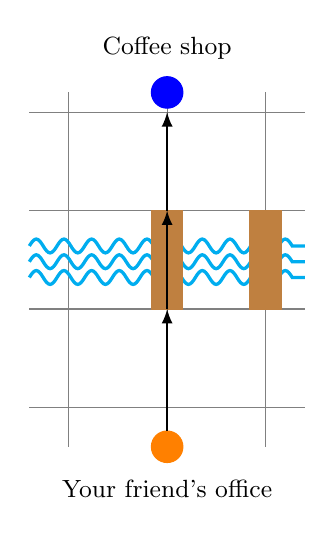
\begin{tikzpicture}
    \draw[step=\stepgrid cm,color=gray] (\startlowleft,\startlowleft) grid (\stoplowright,\stophighright);
    % --- Blue circle
    \draw [blue,fill] (2*\stepgrid , \stophighright) circle [radius=0.2] node [black,above=0.3] {Coffee shop};
    % --- Orange circle
    \draw [orange,fill] (2*\stepgrid , \startlowleft) circle [radius=0.2] node [black,below=0.3] {Your friend's office};
    % --- River
    \draw[cyan, very thick, snake=coil,segment aspect=0] (\startlowleft,2*\stepgrid+0.4)   -- (\stoplowright,2*\stepgrid+0.4);
    \draw[cyan, very thick, snake=coil,segment aspect=0] (\startlowleft,2*\stepgrid+0.6)   -- (\stoplowright,2*\stepgrid+0.6);
    \draw[cyan, very thick, snake=coil,segment aspect=0] (\startlowleft,2*\stepgrid+0.8)   -- (\stoplowright,2*\stepgrid+0.8);
    % --- Bridge
    \draw[brown, fill] (2*\stepgrid - 0.2, 2*\stepgrid) rectangle (2*\stepgrid + 0.2, 3*\stepgrid);
    % --- Path
    \draw[->, >=latex, thick] (2*\stepgrid, \startlowleft+0.2)  -- (2*\stepgrid, 2*\stepgrid);
    \draw[->, >=latex, thick] (2*\stepgrid, 2*\stepgrid)  -- (2*\stepgrid, 3*\stepgrid);
    \draw[->, >=latex, thick] (2*\stepgrid, 3*\stepgrid)  -- (2*\stepgrid, 4*\stepgrid);
    % --- New Bridge
    \draw[brown, fill] (3*\stepgrid - 0.2, 2*\stepgrid) rectangle (3*\stepgrid + 0.2, 3*\stepgrid);
    \end{tikzpicture}
  \end{tabular}
  \end{minipage}
\end{document}
